% reset section counter
\setcounter{section}{0}

%\metadata{lecture ID}{Your names}{date}
\metadata{4}{Yizhou Qian}{Jan 25th, 2021}

In Chapter \ref{chap:asymp}, we pointed out some limitations of asymptotic analysis. In this chapter, we will turn our focus to \textit{non-asymptotic analysis}, where we provide convergence guarantees without having the number of observations $n$ go off to infinity. A key tool for proving such guarantees is \textit{uniform convergence}, where we have bounds of the following form:
\al{
 \Pr \left[ \sup_{h \in \cH} \vert \hat L(h) - L(h) \vert \leq \epsilon \right] \geq 1 - \delta.
\label{lec4:eqn:uniformconvergence}
}
In other words, the probability that the difference between our empirical loss and population loss is larger than $\epsilon$ is at most $\delta$. We give motivation for uniform convergence and show how it can give us non-asymptotic guarantees on excess risk.

\sec{Basic concepts}

A central goal of learning theory is to bound the \emph{excess risk} $L(\hat{\theta}) - L(\theta^*)$. This is important as we don't want the expected risk of our ERM to be much larger than the expected risk of the best possible model. As we will see in the remainder of this section, uniform convergence is a technique that helps us achieve such bounds.

Uniform convergence is a property of a parameter set $\Theta$, which gives us bounds of the form
\al{
    \Pr \left[|\hat{L}(\theta) - L(\theta)| \geq \varepsilon \right] \leq \delta; \; \forall \theta \in \Theta.\label{lec2:eqn:uc}
}
In other words, uniform convergence tells us that for any choice of $\theta$, our empirical risk is always close to our population risk with high probability. Let's look at a motivating example for why this type of bound is useful.

\subsec{Motivation: Uniform convergence implies generalization}\label{sec:uc-gen}

Consider the standard supervised learning setup where we have some i.i.d. $(x\sp{i}, y\sp{i})$. Furthermore, assume that we have a bounded loss function; specifically, suppose that $0 \leq \ell((x, y); \theta) \leq 1$, as in the case of the zero-one loss function. We show that uniform convergence implies generalization.

First, via telescoping sums, we can decompose the excess risk into three terms:
\al{
    L(\hat{\theta}) - L(\theta^*) = \underbrace{L(\hat{\theta}) - \hat{L}(\hat{\theta})}_\text{\circled{1}} + \underbrace{\hat{L}(\hat{\theta}) - \hat{L}(\theta^*)}_\text{\circled{2}} + \underbrace{\hat{L}(\theta^*) - L(\theta^*)}_\text{\circled{3}}.
}
We know that $\hat{L}(\hat{\theta}) - \hat{L}(\theta^*) \leq 0$ since $\hat{\theta}$ is a minimizer of $\hat{L}$. This allows us to write
\begin{align}
L(\hat{\theta}) - L(\theta^*) &\leq |L(\hat{\theta}) - \hat{L}(\hat{\theta})| + \hat{L}(\hat{\theta}) - \hat{L}(\theta^*) + |\hat{L}(\theta^*) - L(\theta^*)|\\
&\leq |L(\hat{\theta}) - \hat{L}(\hat{\theta})| + 0 + |\hat{L}(\theta^*) - L(\theta^*)|\\
&\leq 2\;\sup_{\theta \in \Theta } |L(\theta) - \hat{L}(\theta)|. \label{lec2:eqn:1}
\end{align}
This result tells us that if $\sup_{\theta \in \Theta } |L(\theta) - \hat{L}(\theta)|$ is small (say, less than $\varepsilon/2$), then excess risk $L(\hat{\theta}) - L(\theta^*)$ is less than $\varepsilon$. But this is exactly in the form of the bound in \eqref{lec2:eqn:uc}. Hence, if we can show that a parameter family exhibits uniform convergence, we can get a bound on excess risk as well.

For future references, Equation~\eqref{lec2:eqn:1} can be strengthened straightforwardly into the following with slightly more careful treatment of the signs of each term:
\begin{align}
L(\hat{\theta}) - L(\theta^*) \le |\hat{L}(\theta^*) - L(\theta^*)|+  L(\hat{\theta}) - \hat{L}(\hat{\theta})  \le |\hat{L}(\theta^*) - L(\theta^*)|+ \sup_{\theta \in \Theta} \left(L(\theta) - \hat{L}(\theta)\right)\label{lec2:eqn:2}
\end{align}
This will make some of our future derivations technically slightly more convenient, but the nuanced difference between Equations~\eqref{lec2:eqn:1} and~\eqref{lec2:eqn:2} does not change the fundamental idea and the discussions in this chapter. 

Let us try to apply our knowledge of concentration inequalities to this problem. Earlier we assumed that $\ell((x, y); \theta)$ is bounded, so we can bound $\circled{3}$ \todo{replace $\circled{3}$ etc by something that looks more aesthetic} 
by $\tilO\left(\frac{1}{\sqrt{n}}\right)$ via Hoeffding's inequality (Remark \ref{lec2:rem:hoeffding}). However, we cannot apply the same concentration inequality to $\circled{1}$: since $\hat{\theta}$ is data-dependent by definition, the i.i.d. assumption no longer holds. (To see this, note that $\hat\theta$ depends on the training dataset $\{(x\sp{i}, y\sp{i})\}$, so the terms in $\hatL (\hat\theta)$, $\ell ((x\sp{i}, y\sp{i}); \hat\theta)$, all depend on the training dataset too.) This is concerning: it is certainly possible that $L(\hat{\theta}) - \hat{L}(\hat{\theta})$ is large. You've probably encountered this yourself when a model exhibits low training loss, but high validation/testing loss. 

\subsec{Deriving uniform convergence bounds}

Uniform convergence is one way we can control this issue. The high-level idea is as follows: 
\begin{itemize}
    \item Suppose we have a bound of the form $\Pr[|\hat{L}(\theta) - L(\theta)| \geq \varepsilon'] \leq \delta'$ for some single, fixed choice of $\theta$.
    \item If we know \emph{all possible values of $\theta$} in advance, we can use the above bound to create a more general bound over all values of $\theta$.
\end{itemize}
In particular, we can use the union-bound inequality to create the general bound described in the second bullet point, using the bound in the first bullet point:
\al{
    \Pr \left[\forall \theta \in \Theta, |\hat{L}(\theta) - L(\theta)| \geq \varepsilon' \right] \leq \sum_{\theta \in \Theta} \Pr \left[|\hat{L}(\theta) - L(\theta)| \geq \varepsilon' \right].
}
We can then use Hoeffding's inequality to deal with the summands as $\theta$ there is no longer data-dependent. We will talk more later about proving statements of this form.

\subsec{Intuitive interpretation of uniform convergence}

Since uniform convergence implies generalization, if we know that population risk and empirical risk are always ``close," then excess risk is ``small" as well (Figure \ref{lec2:fig:uc}). In fact, it is possible to show that not only is $L(\theta)$ ``close" to $\hat{L}(\theta)$ for sufficiently large data, but that the ``shape" of $\hat{L}$ is ``close" to the shape of $L$ as well (Figure \ref{lec2:fig:shape}). This holds for the convex case; furthermore, there are conditions under which this holds in the non-convex case, for which a rigorous treatment can be found in~\cite{mei2017landscape}. (\emph{Figure design and some wording in this section was inspired by~\cite{percynotes, thomasliu2018}.})

\begin{figure}[t]
    \centering
    \begin{subfigure}[t]{0.49\textwidth}
        \hspace*{0.8em}
        \centering
        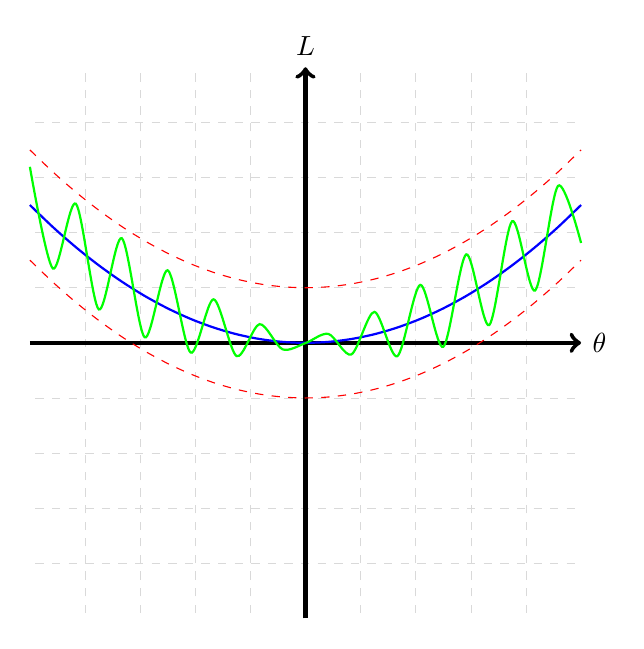
\begin{tikzpicture}[scale=0.7]
            \draw[help lines, color=gray!30, dashed] (-4.9,-4.9) grid (4.9,4.9);
            \draw[->,ultra thick] (-5,0)--(5,0) node[right]{$\theta$};
            \draw[->,ultra thick] (0,-5)--(0,5) node[above]{$L$};
            \draw[blue, thick]   plot[smooth,domain=-5:5] (\x, {0.1* (\x*\x)});
            \draw[red, dashed]   plot[smooth,domain=-5:5] (\x, {0.1* (\x*\x) + 1});
            \draw[red, dashed]   plot[smooth,domain=-5:5] (\x, {0.1* (\x*\x) - 1});
            \draw[green, thick]   plot[smooth,domain=-5:5] (\x, {0.1* (\x*\x) + 0.8 * sin(3000 * \x)});
        \end{tikzpicture}
        \caption{}
        \label{lec2:fig:uc}
    \end{subfigure}
    \hfill
    \begin{subfigure}[t]{0.49\textwidth}
        \hspace*{0.8em}
        \centering
        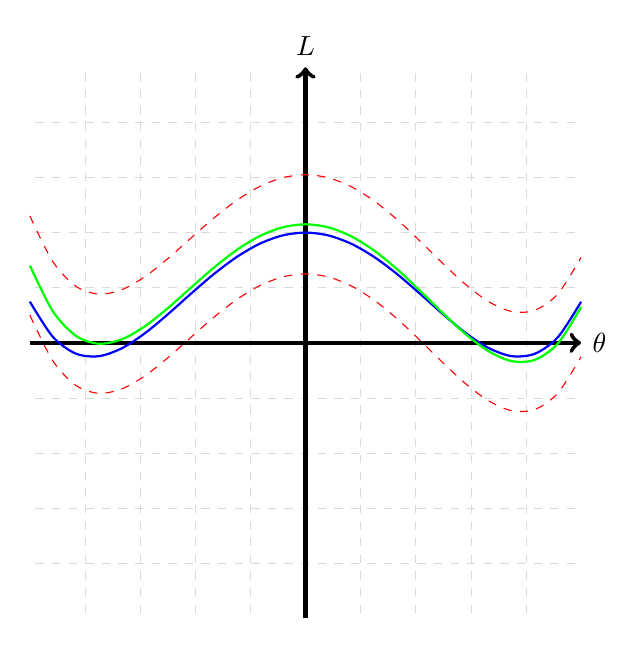
\begin{tikzpicture}[scale=0.7]
            \draw[help lines, color=gray!30, dashed] (-4.9,-4.9) grid (4.9,4.9);
            \draw[->,ultra thick] (-5,0)--(5,0) node[right]{$\theta$};
            \draw[->,ultra thick] (0,-5)--(0,5) node[above]{$L$};
            \draw[blue, thick]   plot[smooth,domain=-5:5] (\x, {0.01*\x*\x*\x*\x - 0.3*\x*\x + 2});
            \draw[green, thick]   plot[smooth,domain=-5:5] (\x, {0.011*\x*\x*\x*\x -0.003*\x*\x*\x - 0.32*\x*\x + 2.15});
            \draw[red, dashed]   plot[smooth,domain=-5:5] (\x, {0.011*\x*\x*\x*\x -0.003*\x*\x*\x - 0.32*\x*\x + 3.05});
            \draw[red, dashed]   plot[smooth,domain=-5:5] (\x, {0.011*\x*\x*\x*\x -0.003*\x*\x*\x - 0.32*\x*\x + 1.25});
        \end{tikzpicture}
        \caption{}
        \label{lec2:fig:shape}
    \end{subfigure}
    \caption{These curves demonstrate how we apply uniform convergence to bound the population risk. The \textcolor{blue}{blue} curves are the unobserved population risk we aim to bound. The \textcolor{green}{green} curves denote the empirical risk we observe. Though this curve is often depicted as the fluctuating curve used in Figure~\ref{lec2:fig:uc}, it is more often a smooth curve whose shape mimics that of the population risk (Figure~\ref{lec2:fig:shape}). Uniform convergence allows us to construct additive error bounds for the excess risk, which are depicted using the \textcolor{red}{red, dashed} lines.}
    \label{lec2:fig:uc_shape}
\end{figure}

\sec{Finite hypothesis class}

In this section, assume that $\cH$ is finite. The following theorem gives a bound for the excess risk $L(\hat{h}) - L(h^{*})$, where $\hat{h}$ and $h^*$ are the minimizers of the empirical loss and population loss respectively.

\begin{theorem}\label{lec4:thm:finite}
Suppose that our hypothesis class $\cH$ is finite and that our loss function $\ell$ is bounded in $[0,1]$, i.e. $0 \leq \ell((x, y), h) \leq 1$. Then $\forall \delta \  s.t. \  0 < \delta < \frac{1}{2}$ , with probability at least $1 - \delta$, we have 
\al {
\vert L(h) - \hat{L}(h) \vert \leq \sqrt{\frac{\ln{\vert \cH \vert} + \ln{(2 / \delta)}}{2n}} \qquad \forall h \in \cH.
\label{lec4:eqn:finiteuniformbound}
}
As a corollary, we also have 
\al {
L(\hat{h}) - L(h^{*}) \leq \sqrt{\frac{ 2(\ln{\vert \cH \vert} + \ln{(2 / \delta)}) }{n}}.
\label{lec4:eqn:finiteexcessriskbound}
}
\end{theorem}

\begin{proof}
We will prove this in two steps:
\begin{enumerate}
\item Use concentration inequalities to prove the bound for a fixed $h \in \cH$, then
\item Use a union bound across the $h$'s. (Recall that if $E_1, \dots, E_k$ are a finite set of events, then the union bound states that $\Pr ( E_1 \cup \dots \cup E_k) \leq \sum_{i = 1}^k \Pr(E_i)$.)
\end{enumerate}

Fix some $\epsilon > 0$. By applying Hoeffding's inequality on the $\ell( (x\sp{i}, y\sp{i}), h)$, we know that 

\al{
\Pr \left( \vert \hat{L}(h) - L(h) \vert \geq \epsilon \right) &\leq 2\exp\left(-\frac{2n^2\epsilon^2}{\sum_{i = 1}^n(b_i - a_i)^2}\right) \\
&= 2\exp\left(-\frac{2n^2\epsilon^2}{n}\right) \\
&= 2\exp(-2n\epsilon^2),
\label{lec4:eqn:boundedconcentration}
}
since we can set $a_i = 0, b_i = 1$. The bound above holds for a single fixed $h$. To prove a similar inequality that holds for all $h \in \cH$, we apply the union bound with $E_h = \{\vert \hat{L}(h) - L(h) \vert \geq \epsilon \}$:
\al{
\Pr \left( \exists h \text{ s.t. } \vert \hat{L}(h) - L(h) \vert \geq \epsilon \right) &\leq \sum_{h \in \cH} \Pr \left(\vert \hat{L}(h) - L(h) \vert \geq \epsilon \right) \\
&\leq \sum_{h \in \cH} 2\exp(-2n\epsilon^2) \\
&= 2\vert \cH \vert \exp(-2n\epsilon^2). 
\label{lec4:eqn:unionboundforh}
}
If we take $\delta$ such that $2\vert \cH \vert \exp(-2n\epsilon^2) = \delta$, then it follows that 
\al {
\epsilon = \sqrt{\frac{\ln{\vert \cH \vert} + \ln{(2 / \delta)}}{2n}},
\label{lec4:eqn:probabilitytoerror}
}
which proves \eqref{lec4:eqn:finiteuniformbound}. \eqref{lec4:eqn:finiteexcessriskbound} follows by the inequality we stated in Section \ref{sec:uc-gen} and taking 
\begin{align}
    \epsilon = \sqrt{\frac{ 2(\ln{\vert \cH \vert} + \ln{(2 / \delta)}) }{n}},
\end{align}
we have that
\begin{align}
\Pr \left( | L(\hat{h}) - L(h^{*}) | \geq \epsilon \right) &\leq \Pr \left( 2 \sup_{h \in \cH} | \hat{L}(h) - L(h) | \geq \epsilon \right) \\
&\leq 2 |\cH| \exp \left( -\frac{n\epsilon^2}{2} \right).
\end{align}
\end{proof}

\subsec{Comparing Theorem \ref{lec4:thm:finite} with standard concentration inequalities}
With standard concentration inequalities, we have the following bound that depends on empirical risk:
\al{
\forall h \in \cH, \quad w.h.p. \quad \vert \hat{L}(h) - L(h) \vert \leq \tilde{O} \left( \frac{1}{\sqrt{n}} \right).
\label{lec4:eqn:centrallimitconvergence}
}
The bound here depends on each $h$. In contrast, the uniform convergence bound we obtain from \eqref{lec4:eqn:probabilitytoerror} is uniform over all $h \in \cH$:
\al{
w.h.p., \quad \forall h \in \cH, \quad \vert \hat{L}(h) - L(h) \vert \leq \tilde{O} \left( \frac{ \ln |\cH|}{\sqrt{n}} \right),
}
if we omit the $\ln{(1/\delta)}$ factor (we can do this since $\ln{(1/\delta)}$ is small in general and we take $\delta = \frac{1}{poly(n)}$). Hence, the extra $\ln{\vert \cH \vert}$ term that depends on the size of our finite hypothesis family $\cH$ can be viewed as a trade-off in order to make the bound uniform.

\begin{remark}
There is no standard definition for the term \textit{with high probability} (\textit{w.h.p}). For this class, the term is equivalent to the condition that the probability is higher than $1 - n^{-c}$ for some constant $c$.
\end{remark}

\subsec{Comparing Theorem \ref{lec4:thm:finite} with asymptotic bounds}
We can also compare the bound in Theorem \ref{lec4:thm:finite} with our original asymptotic bound, namely,
\al{
L(\hat{h}) - L(h^*) \leq \frac{c}{n} + o \left(n^{-1} \right).
\label{lec4:eqn:asymptotics}
}
The $o(n^{-1})$ term can vary significantly depending on the problem. For instance, both $n^{-2}$ and $p^{100}n^{-2}$ are $o(n^{-1})$ but the second one converges much more slowly. With the new bound, there are no longer any constants hidden in an $o(n^{-1})$ term (in fact that term is no longer there). However, we now have a slower convergence rate of $O(n^{-1/2})$.

\begin{remark}
$O(n^{-1/2})$ convergence is sometimes known as the \textit{slow rate} while $O(n^{-1})$ convergence is known as the \textit{fast rate}. We were only able to get the slow rate from uniform convergence: we needed asymptotics to get the fast rate. (It is possible to get the fast rate from uniform convergence under certain conditions, e.g. when the population risk on the true $h^*$ is very low.)
\end{remark}

\sec{Bounds for infinite hypothesis class via discretization}
Unfortunately, we cannot generalize the results from the previous section directly to the case where the hypothesis class $\cH$ is infinite, since we cannot apply the union bound to an infinite number of hypothesis functions $h \in \cH$. However, if we consider a \emph{bounded} and \emph{continuous} parameterized space of $\cH$, then we can obtain a similar uniform bound by applying a technique called \emph{brute-force discretization}.

For this section, assume that our infinite hypothesis class $\cH$ can be parameterized by $\theta \in \mathbb{R}^p$ with $\Vert \theta \Vert_2 \leq B$ for some fixed $B > 0$. That is, we have 
\al{
\cH = \{h_{\theta} : \theta \in \mathbb{R}, \Vert \theta \Vert_2 \leq B \}.
\label{lec4:eqn:infiniteclass}
}

The intuition behind brute-force discretization is as follows: Let $E_\theta = \{ |\hatL(\theta) - L(\theta)| \geq \epsilon \}$ be the ``bad" event. We want the bound the probability of any one of these bad events happening (i.e. $\bigcup_\theta E_\theta$). The union bound does not work as we end up with an infinite sum. However, the union bound is very loose: these events can overlap with each other significantly. Instead, we can try to find ``prototypical" bad events $E_{\theta_1}, \dots, E_{\theta_N}$ that are somewhat disjoint so that $\bigcup_\theta E_\theta \approx \bigcup_{i=1}^N E_{\theta_i}$. We can then use the union bound on $\bigcup_{i=1}^N E_{\theta_i}$ to get a non-vacuous upper bound.

We make these ideas precise in the following section.

\subsec{Discretization of the parameter space by \texorpdfstring{$\epsilon$}{epsilon}-covers}

We start by defining the notion of an \emph{$\epsilon$-cover} (also \textit{$\epsilon$-net}):

\begin{definition}[$\epsilon$-cover]
Let $\epsilon>0$. An \emph{$\epsilon$-cover} of a set $S$ with respect to distance metric $\rho$ is a subset $C \subseteq S$ such that $\forall x \in S$, $\exists x' \in C$ such that $\rho(x,x') \le \epsilon$, or equivalently,
\begin{align}
S &\subseteq \bigcup_{x \in C} \mathrm{Ball}(x, \epsilon, \rho), \quad \text{where} \\
\mathrm{Ball}(x, \epsilon, \rho) &\triangleq \{ x': \rho(x, x') \leq \epsilon \}.
\end{align}
\end{definition}

(We note that in some definitions it is possible for points in $C$ to lie outside of $S$; we do not worry about this technicality the class.) The following lemma tells us that our parameter space $S = \{\theta \in \R^p: \|\theta\|_2 \le B\}$ has an $\epsilon$-cover with not too many elements:

\begin{lemma}[$\epsilon$-cover of $\ell_2$ ball]\label{lec4:lem:ECSize}
Let $B,\epsilon>0$, and let $S = \{x \in \R^p: \|x\|_2 \le B\}.$ Then there exists an $\epsilon$-cover of $S$ with respect to the $\ell_2$-norm with at most $\max \left (\left(\frac{3B\sqrt{p}}{\epsilon}\right)^p, 1 \right)$  elements.
\end{lemma}

\begin{proof}
Note that if $\epsilon > B\sqrt{p}$, then $S$ is trivially contained in the ball centered at the origin with radius $\epsilon$ and the $\epsilon$-cover has size 1. Assume $\epsilon \leq B \sqrt{p}$. Set
\begin{equation}
C = \left\{ x \in S: x_i = k_i \frac{\epsilon}{\sqrt{p}}, k_i \in \mathbb{Z}, |k_i| \leq  \frac{B\sqrt{p}}{\epsilon}  \right\},
\end{equation}
i.e. $C$ is the set of grid points in $\R^p$ of width $\tfrac{\epsilon}{\sqrt{p}}$ that are contained in $S$. See Figure \ref{lec5:fig:ecover} for an illustration. 
\begin{figure}[ht]
\centerline{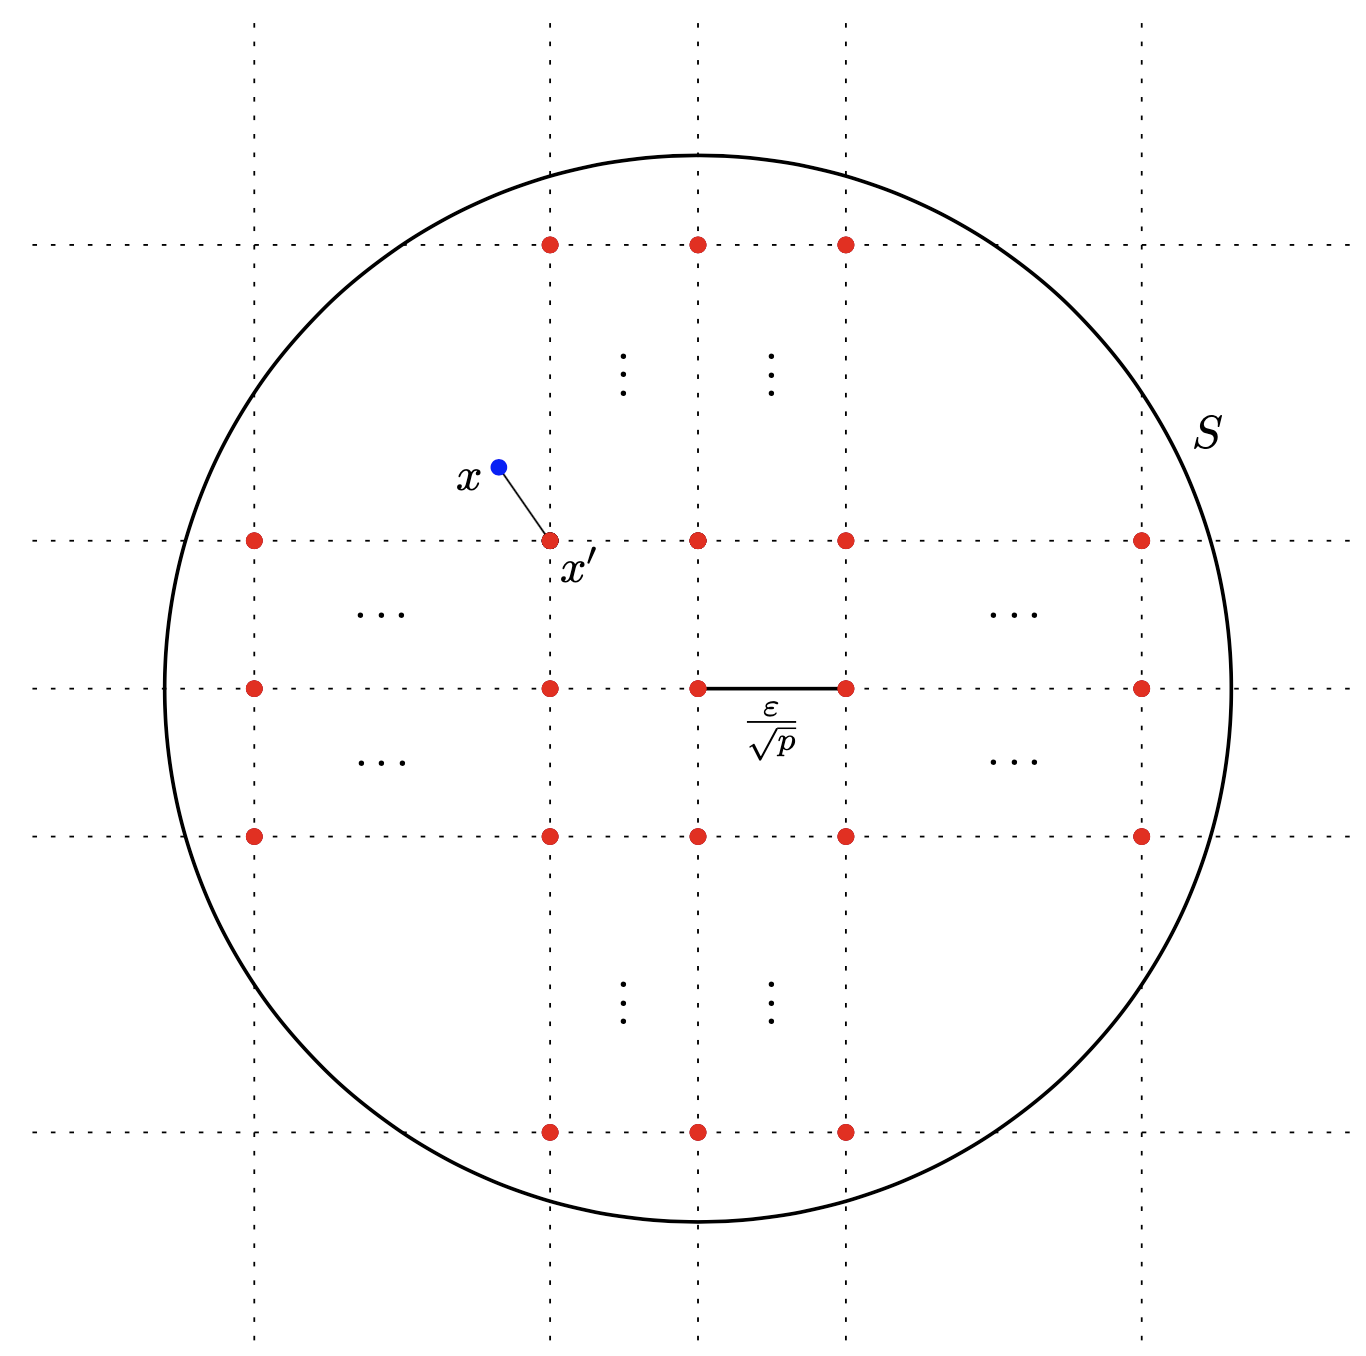
\includegraphics[width=3in]{figures/ECover.png}}
\caption[lec5:fig:ecover]{The $\epsilon$-cover (shown in red) of $S$ we construct in the proof of Lemma~\ref{lec4:lem:ECSize}. For $x \in S$, we choose the grid point $x'$ such that $\norm{x-x'}_2 \le \epsilon$.}
\label{lec5:fig:ecover}
\end{figure}

We claim that $C$ is an $\epsilon$-cover of $S$ with respect to the $\ell_2$-norm: $\forall x \in S$, there exists a grid point $x' \in C$ such that $|x_i-x_i'| \le \tfrac{\epsilon}{\sqrt{p}}$ for each $i$. Therefore,
$$\norm{x-x'}_2 = \sqrt{\sum_{i = 1}^p |x_i - x_i'|^2} \leq \sqrt{p\cdot \frac{\epsilon^2}{p}} = \epsilon.$$

We now bound the size of $C$. Since each $k_i$ in the definition of $C$ has at most $2\tfrac{B\sqrt{p}}{\epsilon}+1$ choices, we have 
\begin{equation}
|C| \le \left( \frac{2B\sqrt{p}}{\epsilon} +1\right)^p \le \left(\frac{3B\sqrt{p}}{\epsilon}\right)^p.
\end{equation}
\end{proof}

\begin{remark}\label{lec4:rem:enet}
We can actually prove a stronger version of Lemma \ref{lec4:lem:ECSize}: there exists an $\epsilon$-cover of $S$ with at most $\left(\frac{3B}{\epsilon}\right)^p$ elements. We will be using this version of the lemma in the proof below. (We will leave the proof of this stronger version as a homework exercise.)
\end{remark}

\subsec{Uniform convergence bound for infinite \texorpdfstring{$\cH$}{H}}

\begin{definition}[$\kappa$-Lipschitz functions]
Let $\kappa \ge 0$ and $\norm{\cdot}$ be a norm on the domain $D$. A function $L:D \to \R$ is said to be \emph{$\kappa$-Lipschitz} with respect to $\norm{\cdot}$ if for all $\theta, \theta' \in D$, we have
$$
    |L(\theta)-L(\theta')| \le \kappa \norm{\theta-\theta'}.
$$
\end{definition}

Assume that our infinite hypothesis class $\cH$ can be parameterized by $\cH = \{h_{\theta} : \theta \in \mathbb{R}, \Vert \theta \Vert_2 \leq B\}$. We have the following uniform convergence theorem for our infinite hypothesis class $\cH$:

\begin{theorem}\label{lec4:thm:main}
Suppose $\ell((x,y), \theta) \in [0,1]$, and $\ell((x,y), \theta)$ is $\kappa$-Lipschitz in $\theta$ with respect to the $\ell_2$-norm for all $(x, y)$. Then, with probability  at least $1-O(\exp(-\Omega(p)))$, we have
\begin{equation}
    \forall \theta, \quad |\hat L(\theta)- L(\theta)| \leq  O\left(\sqrt{\frac{p \max(\ln{(\kappa Bn), 1)}}{n}}\right).
\end{equation}
\end{theorem}

\begin{proof}[Proof of Theorem \ref{lec4:thm:main}]
Fix parameters $\delta, \epsilon>0$ (we will specify their values later). Let $C$ be the $\epsilon$-cover of our parameter space $S$ with respect to the $\ell_2$-norm constructed in Lemma \ref{lec4:lem:ECSize}. Define event $E = \left\{ \forall \theta \in C, \; |\hat L(\theta) - L(\theta)| \le \delta \right\}$. By Theorem 4.1, we have $\Pr (E) \ge 1 - 2|C|\exp(-2n\delta^2)$.

Now for any $\theta \in S$, we can pick some $\theta_0 \in C$ such that $\norm{\theta-\theta_0}_2 \le \epsilon$. Since $L$ and $\hatL$ are $\kappa$-Lipschitz functions (this follows from the Lipschitzness of $\ell$), we have
\begin{align}
|L(\theta) - L(\theta_0)| &\le \kappa \norm{\theta-\theta_0}_2 \le \kappa \epsilon, \text{ and} \\
|\hat L(\theta) - \hat L(\theta_0)| &\le \kappa \norm{\theta-\theta_0}_2 \le \kappa \epsilon.
\end{align}

Therefore, conditional on $E$, we have
\begin{equation}
    |\hat L(\theta) -  L(\theta)| \le |\hat L(\theta)-\hat L(\theta_0)| + |\hat L(\theta_0) -  L(\theta_0)| + | L(\theta_0) - L(\theta)| \le 2 \kappa\epsilon+\delta.
\end{equation}

It remains to choose suitable parameters $\delta$ and $\epsilon$ to get the desired bound in Theorem \ref{lec4:thm:main} while making the failure probability small. First, set $\epsilon = \delta / (2 \kappa)$ so that conditional on $E$,
\begin{equation} \label{lec4:eqn:triangle}
    |\hat L(\theta) -  L(\theta)| \le 2\delta.
\end{equation}

To choose the correct $\delta$, we must reason about the probability of $E$ under different choices of the parameter. The event $E$ happens with probability $1 - 2|C|\exp(-2n\delta^2) = 1 - 2 \exp(\ln{|C|} - 2n\delta^2)$. From Remark \ref{lec4:rem:enet}, we know that $\ln{|C|} \leq p \ln{ (3B / (\delta / 2)) }$. If we ignore the log term and assume $\ln{|c|} \leq p$, then this would give us the high probability bound we want:
\al{
   2|C| \exp(-2n\delta^2)  = 2\exp(\ln{\vert C \vert} - 2n\delta^2) \leq 2\exp(p - 2p) = 2\exp(-p).
}
(At the same time, we see from \eqref{lec4:eqn:triangle} that this choice of $\delta$ gives $|\hat L(\theta)- L(\theta)| \le 2 \sqrt{\frac{p}{n}}$, which is roughly the bound we want.)

Since we cannot actually drop the log term in the inequality $\ln{|C|} \leq p \ln{ (3B / (\delta / 2)) }$, we need to make $\delta$ a little big bigger. So, if we set $\delta = \sqrt{\frac{c_0 p \max(1, \ln{(\kappa Bn)})}{n}}$ with $c_0 = 36$, then by Remark \ref{lec4:rem:enet},
\begin{align}
\ln{\vert C \vert} - 2n\delta^2 &\leq p \ln\left(\frac{6B \kappa}{\delta}\right) - 2n\delta^2 \\
&\leq p \ln\left(\frac{6B\kappa \sqrt{n}}{ \sqrt{c_0 p \max(1, \ln{(\kappa Bn)})} }\right) - 2n \frac{c_0p}{n} \ln(\kappa Bn) &(\text{dfn of } \delta)  \\
&\leq p\ln\left(\frac{B\kappa \sqrt{n}}{\sqrt{p}}\right) - 72 p \ln(\kappa Bn) &(\max(1, \ln{(\kappa Bn)}) \geq 1, c_0 = 36) \\
&\leq p \ln(B\kappa n) - 72 p \ln(B\kappa n) &(\sqrt{n/p} \leq n) \\
&\leq -p,
\end{align}
since $\ln (B\kappa n) \geq 1$ for large enough $n$. Therefore, with probability greater than $1 - 2|C| \exp(-2n\delta^2) = 1 - 2 \exp(\ln{|C|} - 2n\delta^2) \geq 1 - O(e^{-p})$, we have
\al{
\vert \hat L(\theta) - L(\theta) \vert \leq 2\delta = O\left(\sqrt{\frac{p}{n}\max(1,\ln(\kappa Bn))}\right).
}
\end{proof}

\begin{remark}
We bounded the generalization error $\vert \hat L(\theta) - L(\theta) \vert$ by $\delta + 2\epsilon \kappa \leq \sqrt{\frac{\ln{\vert C \vert}}{n}} + 2\epsilon \kappa$. The term $2\epsilon \kappa$ represents the error from our brute-force discretization. It is not a problem because we can always choose $\epsilon$ small enough without worrying about the growth of the first term $\sqrt{\frac{\ln{\vert C \vert}}{n}}$. This in turn is because $\ln{\vert C \vert} \approx p\ln{\epsilon^{-1}}$, which is very insensitive to $\epsilon$, even if we let $\epsilon = \frac{1}{poly(n)}$. We also observe that both $\sqrt{\frac{\ln{\vert C \vert}}{n}}$ and $\sqrt{\frac{p}{n}}$ are bounds that depend on the ``size" of our hypothesis class, in terms of either its total size or dimensionality. This possibly explains why one may need more training samples when the hypothesis class is larger.
\end{remark}
